\documentclass[11pt,a4paper]{article}
\usepackage{amsmath,amssymb,amsthm,graphicx,hyperref,booktabs}
\usepackage[margin=2.3cm]{geometry}
\newtheorem{theorem}{Theorem}
\newtheorem{proposition}[theorem]{Proposition}
\newtheorem{lemma}[theorem]{Lemma}
\theoremstyle{remark}\newtheorem{remark}[theorem]{Remark}
\graphicspath{{../FIGURES/}}

\title{Daughter spacetimes from regular black holes in higher-dimensional gravity:\\
global structure, collapse beyond idealisation, collider production and tests}
\author{Project Baby Universe --- Genesis Branch}
\date{29 October 2026}

\begin{document}
\maketitle

\begin{abstract}
We study a single, consistent higher-dimensional theory in which ordinary matter can produce a spacetime region that is causally
disconnected from its parent: $D=4+n$ dimensional Einstein gravity with large extra dimensions (fundamental scale $M_D$) supplemented by
the infinite tower of quasi-topological curvature corrections of Bueno, Cano and Hennigar, which removes the black-hole singularity.
(i)~The collapse of a dust ball is glued exactly to the regular static exterior; its maximal extension is curvature-bounded (with a
mass-independent bound $K\,l^4\simeq 188$ in $D=10$), regular at both horizons and geodesically complete, and contains a white-hole region
and a new asymptotically flat universe outside $J^-(\mathcal I^+)$ of the parent, together with a finite closed daughter (the bounced
interior, whose volume grows by up to $10^{115}$ for a stellar collapse).
(ii)~Every closed universe in the theory bounces at $a\geq l$ for any perfect fluid; matter interiors accelerate only for
$N\simeq\frac{D-3}{D-1}\ln(a_{\max}/l)$ e-folds, so lasting inflation would need a vacuum as dense as the hole.
(iii)~An energy-conserving hydrodynamics code built on the generalised Misner--Sharp equations reproduces the exact bounce to $10^{-5}$ and
shows that, with pressure, inhomogeneity and shocks, a horizon forms and the matter bounces in an untrapped core with bounded curvature; in
realistic collapse the bounced core meets the envelope at the inner horizon, and in some runs enters the white-hole region through a throat.
(iv)~With real parton distributions, a $100$\,TeV collider produces such holes iff the horizon threshold lies between $\sim9$\,TeV (LHC) and
$\sim50$\,TeV; they form a trapped surface in $10^{-28}$\,s, evaporate in $10^{-26}$\,s toward a zero-temperature remnant, and the trapped
region never closes, so the daughter survives. Near threshold the holes emit almost nothing and the remnant carries $\sim95\%$ of the energy.
All key formulas and numbers are independently re-derived (Appendix~\ref{app:audit}).
\end{abstract}

\section{Introduction}
Whether a laboratory process could create a new, causally disconnected spacetime region is a question about two things at once: the
behaviour of gravity at high curvature, and the energy at which gravity becomes strong. In general relativity (GR) the first is blocked by
singularity theorems (an inflating region in an asymptotically flat spacetime must have a singularity in its past \cite{FG87}) and the second
by the Planck scale. We work in a framework that removes both obstacles within one action, and ask, in turn: does a daughter spacetime
exist globally; does it survive realistic collapse; can a collider make it; and what could be measured.

\section{Model U}
\subsection{Action and spherical sector}
The theory is $D$-dimensional gravity with an infinite tower of quasi-topological densities \cite{BCH24}. Its spherically symmetric sector
has second-order equations, a Birkhoff theorem and Israel-type junction conditions \cite{BCHM25a,BCHM25b}, and is controlled by one
function $h$ through the generalised Misner--Sharp relation
\begin{equation}
h(\psi)=\frac{\mu}{r^{D-1}},\qquad \psi=\frac{1-(\nabla r)^2}{r^2},\qquad \mu=\frac{16\pi G_D M}{(D-2)\Omega_{D-2}} .
\end{equation}
We use the Hayward tower $h=\psi/(1-\alpha\psi)$ and the Dymnikova-type tower $h=-\ln(1-\alpha\psi)/\alpha$; both bound
$\psi<1/\alpha\equiv1/l^2$. For closed FRW regions $\psi=H^2+1/a^2$ and the generalised Friedmann equation reads
$h(H^2+1/a^2)=16\pi G_D\rho/((D-1)(D-2))$ \cite{BCHMV25}.

\subsection{Regular black holes}
The static solution $f=1-r^2\psi$ has a de Sitter core $f\simeq1-r^2/l^2$ and two horizons above the extremal mass; for the Hayward tower
\begin{equation}
\mu_{\rm ext}=l^{D-3}\Big(\tfrac{D-1}{D-3}\Big)^{\frac{D-1}{2}}\tfrac{D-3}{2},\qquad
T=\frac{(D-3)r_+^2-(D-1)l^2}{4\pi r_+^3},
\end{equation}
so evaporation ends at a zero-temperature remnant.

\subsection{Large extra dimensions}
With $G_D=1/M_D^{n+2}$ (Dimopoulos--Landsberg convention \cite{DL01}) and $l=c_l/M_D$, the extra dimensions have radius
$R=(M_P^2/M_D^{n+2})^{1/n}/2\pi$, $10^3$--$10^6$ times larger than $1/M_D$: collider holes are $D$-dimensional and asymptotically flat. The
horizon threshold is $M_{\rm ext}=\kappa_n c_l^{\,n+1}M_D$ with $\kappa_n=32$--$56$ (Hayward) or $13$--$17$ (Dymnikova) for $n=4$--$7$.

\section{The global daughter spacetime}
\begin{proposition}[Exact gluing]
A closed dust ball of mass parameter $C$ and boundary angle $\chi_b$ glued to the static exterior with $\mu=C\sin^{D-1}\chi_b$ satisfies
$f(R)+\dot R^2=\cos^2\chi_b$: its surface is a radial geodesic of the exterior with energy $E=\cos\chi_b$.
\end{proposition}
The maximal extension of the exterior is tiled by patches I (parent) $\to$ II (black hole) $\to$ III (de Sitter core) $\to$ IV (white hole)
$\to$ I$'$ (new universe), matched through the finite null coordinate (Fig.~\ref{fig:global}).
\begin{proposition}[Global properties]
(a) $\max K\,l^4$ is independent of the mass over $\mu=10^{-3}$--$10^8$: $29$--$34$ ($D=4$), $45$--$48$ ($D=5$), $188$ (Hayward, $D=10$),
$919$ (Dymnikova, $D=10$); the closed interior peaks at the de Sitter value $2D(D-1)/l^4$. (b) At both horizons the Kruskal metric
function has equal finite non-zero limits from both sides. (c) Radial and non-radial, timelike and null geodesics cross every region in
finite affine parameter and never terminate. (d) For $\mu>\mu_{\rm ext}$ the surface reaches I$'$ in finite proper time ($2.5$--$35\,l$);
for $\mu<\mu_{\rm ext}$ it bounces back into the parent.
\end{proposition}
The region IV\,$\cup$\,I$'$ lies outside $J^-(\mathcal I^+)$ of the parent, has its own null infinity and ADM mass $\mu$; the bounced closed
interior is a finite daughter whose volume grows by $(a_{\max}/l)^{D-1}$: $1.3\times10^5$ ($C=10^4$, $D=10$) to $8\times10^{114}$ for a
four-dimensional stellar collapse.

\begin{figure}[t]\centering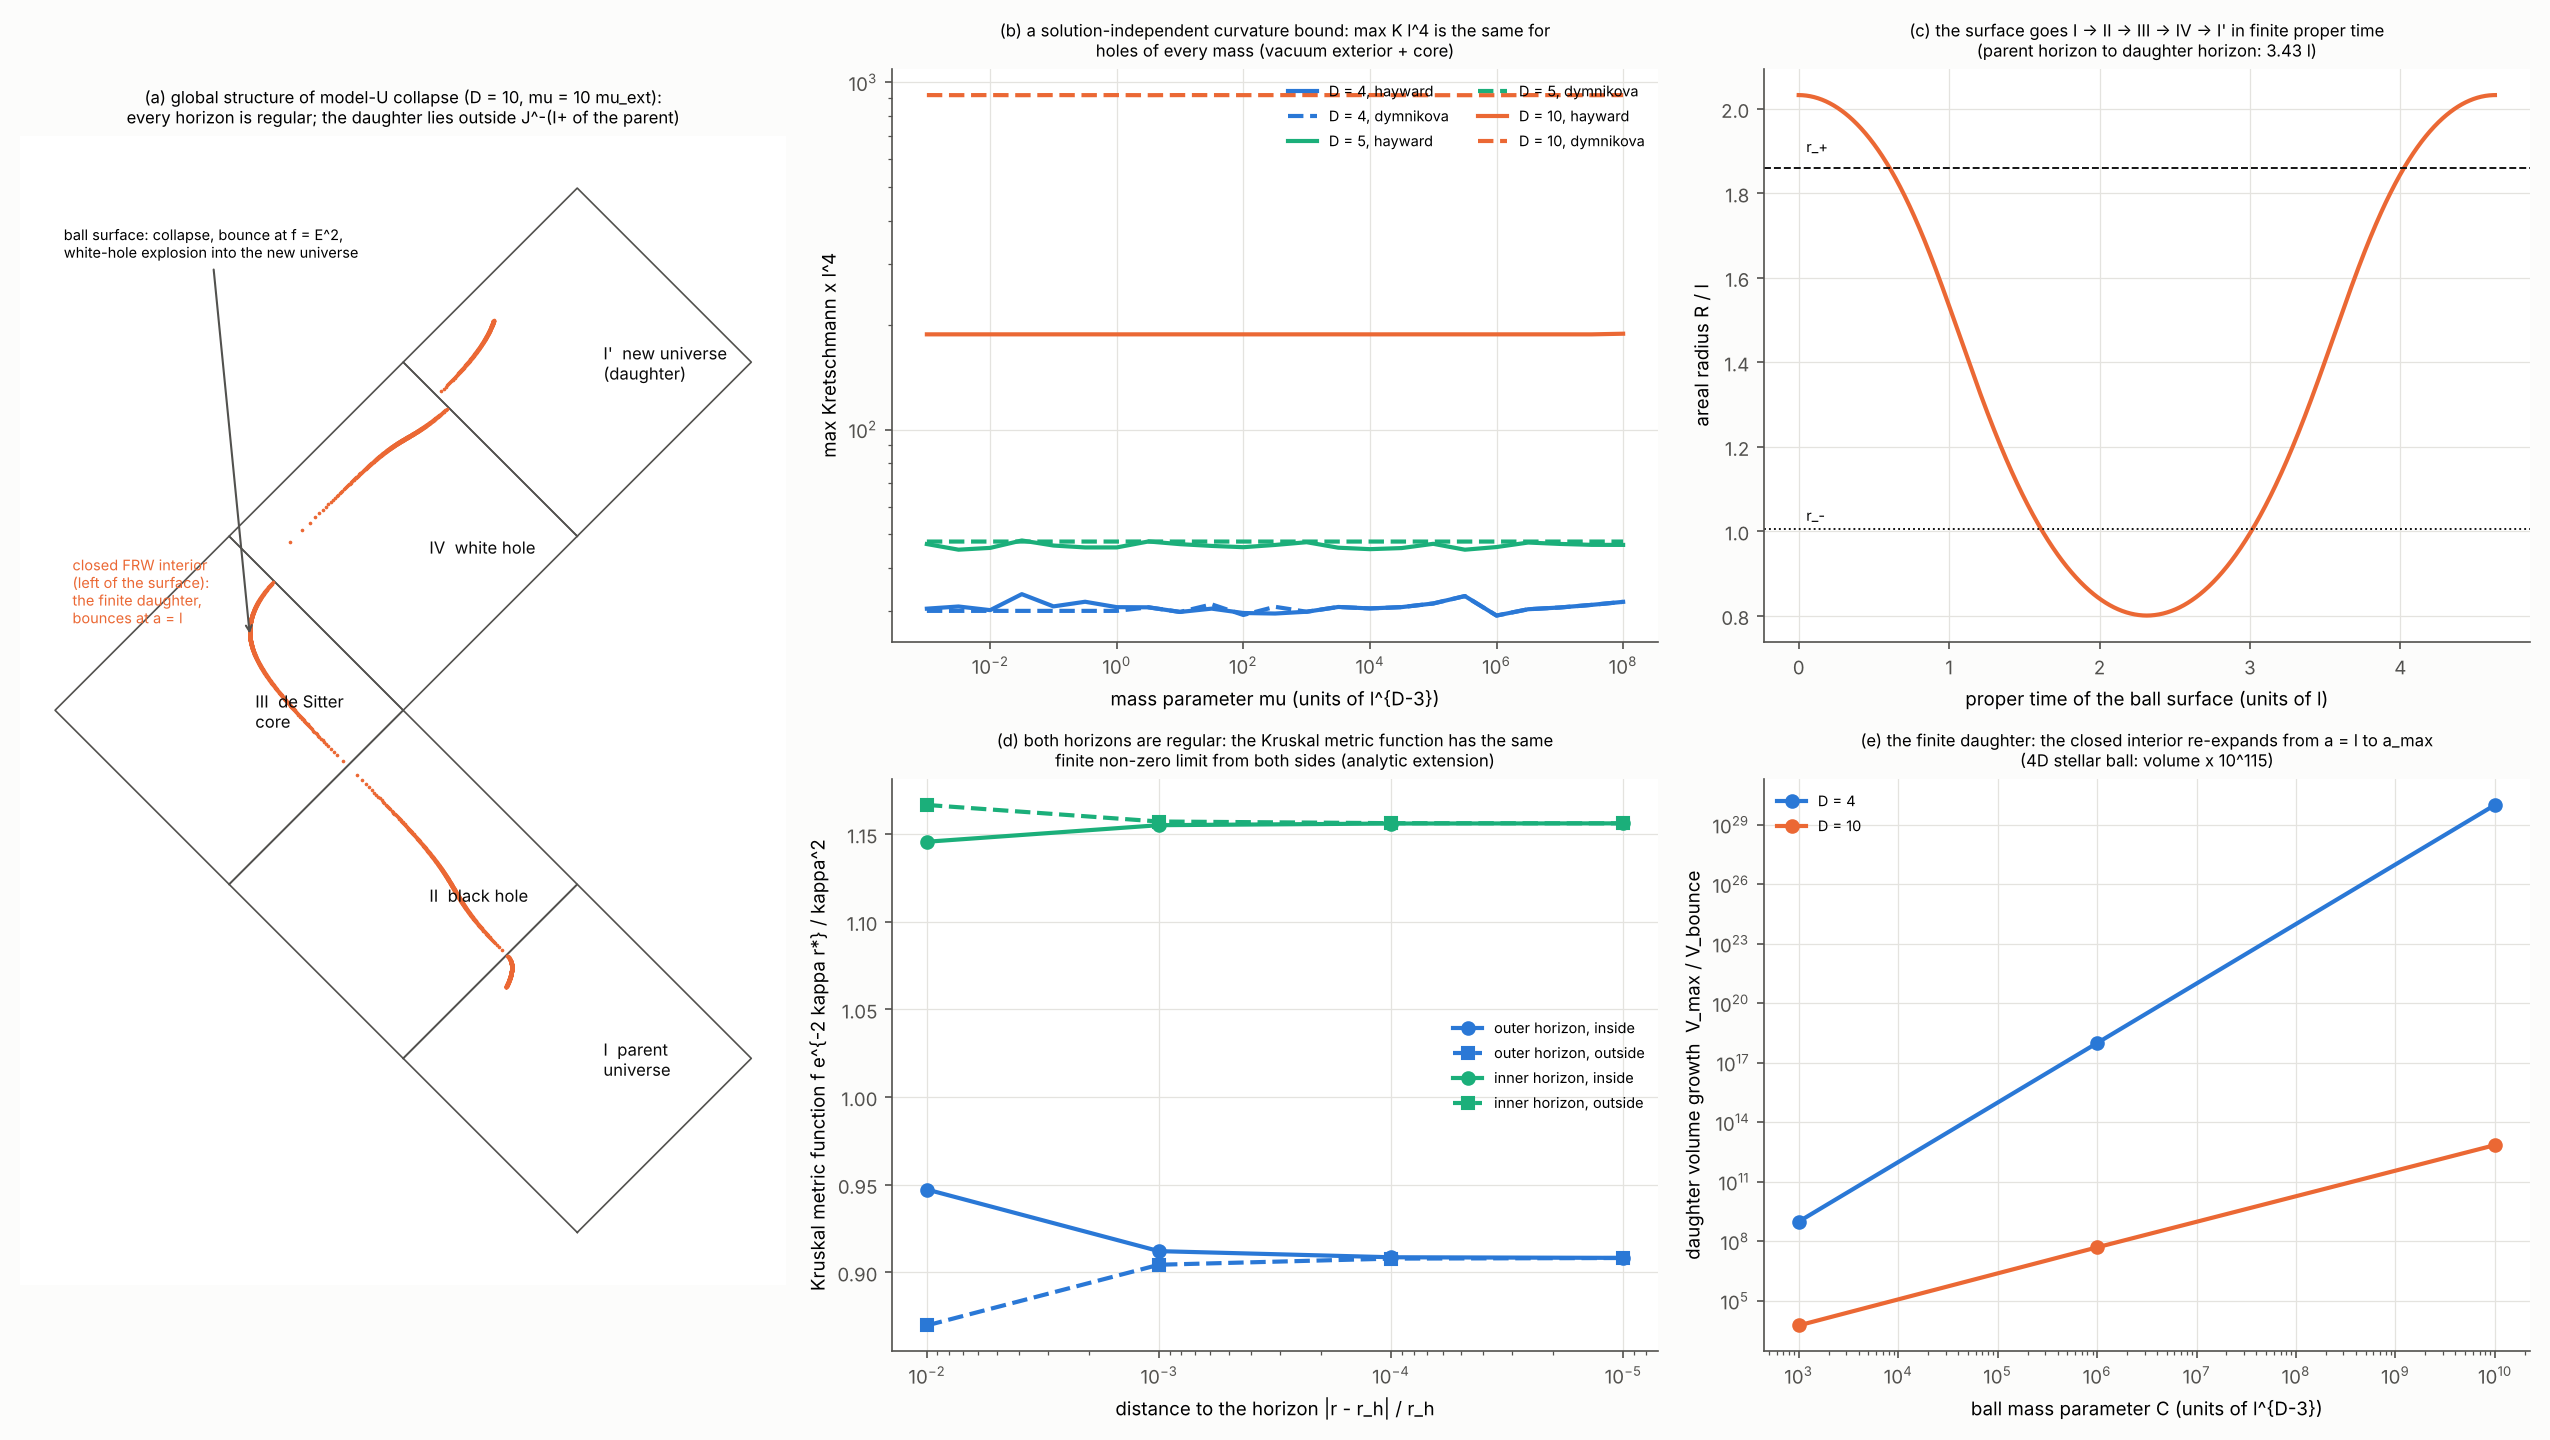
\includegraphics[width=\textwidth]{round6m.png}
\caption{Global structure (Round 6m): (a) Penrose patches with the ball surface; (b) mass-independent curvature bound; (c) radius history;
(d) Kruskal regularity at both horizons; (e) the finite daughter's volume growth.}\label{fig:global}\end{figure}

\section{Interiors}
\begin{proposition}[Universal bounce]
In a closed FRW region with any perfect fluid, $\dot a^2=a^2\psi-1<0$ for $a<l$, so every closed universe bounces at $a_b\geq l$.
\end{proposition}
For dust the turning points coincide with the static horizon radii; the interior accelerates for $N=\ln(a_{\rm infl}/a_b)$ e-folds with
$a_{\rm infl}^{D-1}=2\alpha C/(D-3)$ (Hayward), i.e.\ $N\to\frac{D-3}{D-1}\ln\frac{a_{\max}}{l}+\frac{1}{D-1}\ln\frac{2}{D-3}$ ($29.6$ for a stellar
hole), then decelerates and recollapses. With a vacuum term $\Lambda$ it inflates for ever iff $\Lambda>\Lambda_c(C)$,
$\Lambda_c=[2(\frac{D-3}{D-1})^{(D-1)/2}/((D-3)C)]^{2/(D-3)}$ in the low-curvature limit.
\begin{lemma}[Untrapped bounce]
At a bounce of a radial timelike worldline, $(\nabla R)^2=(n\!\cdot\!\nabla R)^2\geq0$; a bounce inside a black hole requires an untrapped
core bounded by an inner apparent horizon. (Consequently a homogeneous Einstein--Cartan ball, whose Misner--Sharp mass drops by $99\%$ at the
bounce, cannot sit in a vacuum exterior.)
\end{lemma}

\section{Beyond idealised collapse}
In comoving coordinates with $U=D_\tau R$ and $\Gamma=R'e^{-\lambda}$, the Lovelock structure of the spherical sector gives
$\Gamma^2-U^2=1-R^2\psi(\mu/R^{D-1})$, $\mu'=(D-1)\rho R^{D-2}R'$, $D_\tau\mu=-(D-1)pR^{D-2}U$, $D_\tau\Gamma=-U\Gamma p'/((\rho+p)R')$ and
\begin{equation}
D_\tau U=-\frac{\Gamma^2p'}{(\rho+p)R'}+R\psi-\frac{D-1}{2}R\psi'(y)(y+p),\qquad y=\mu/R^{D-1},
\end{equation}
which reduces to GR and to the generalised Friedmann equation. An energy-conserving Lagrangian scheme with non-homologous artificial
viscosity reproduces the exact bounce to $10^{-5}$. Inhomogeneous dust shells bounce at $R_b=\sqrt{k\alpha}$ (within $2\%$), inner shells
first. With pressure, inhomogeneity and shocks (Fig.~\ref{fig:hydro}) every run forms a horizon and bounces in an untrapped core with
$\psi\le0.994/\alpha$ and exact energy conservation. The bounced core meets the infalling envelope at the inner horizon; in some runs its
outer shells become anti-trapped next to trapped envelope shells with $\Gamma\to0$ between them --- a throat joining the parent's black-hole
region to the daughter's white-hole region. The comoving slicing cannot cross that neck; a characteristic code is needed beyond it.
Null thin shells do not exist in these theories \cite{DKS26}, so thin-shell mass-inflation arguments do not apply; regular cores of
Hayward type can be stabilised by phase-space attractors \cite{BKS21,BPS25}.

\begin{figure}[t]\centering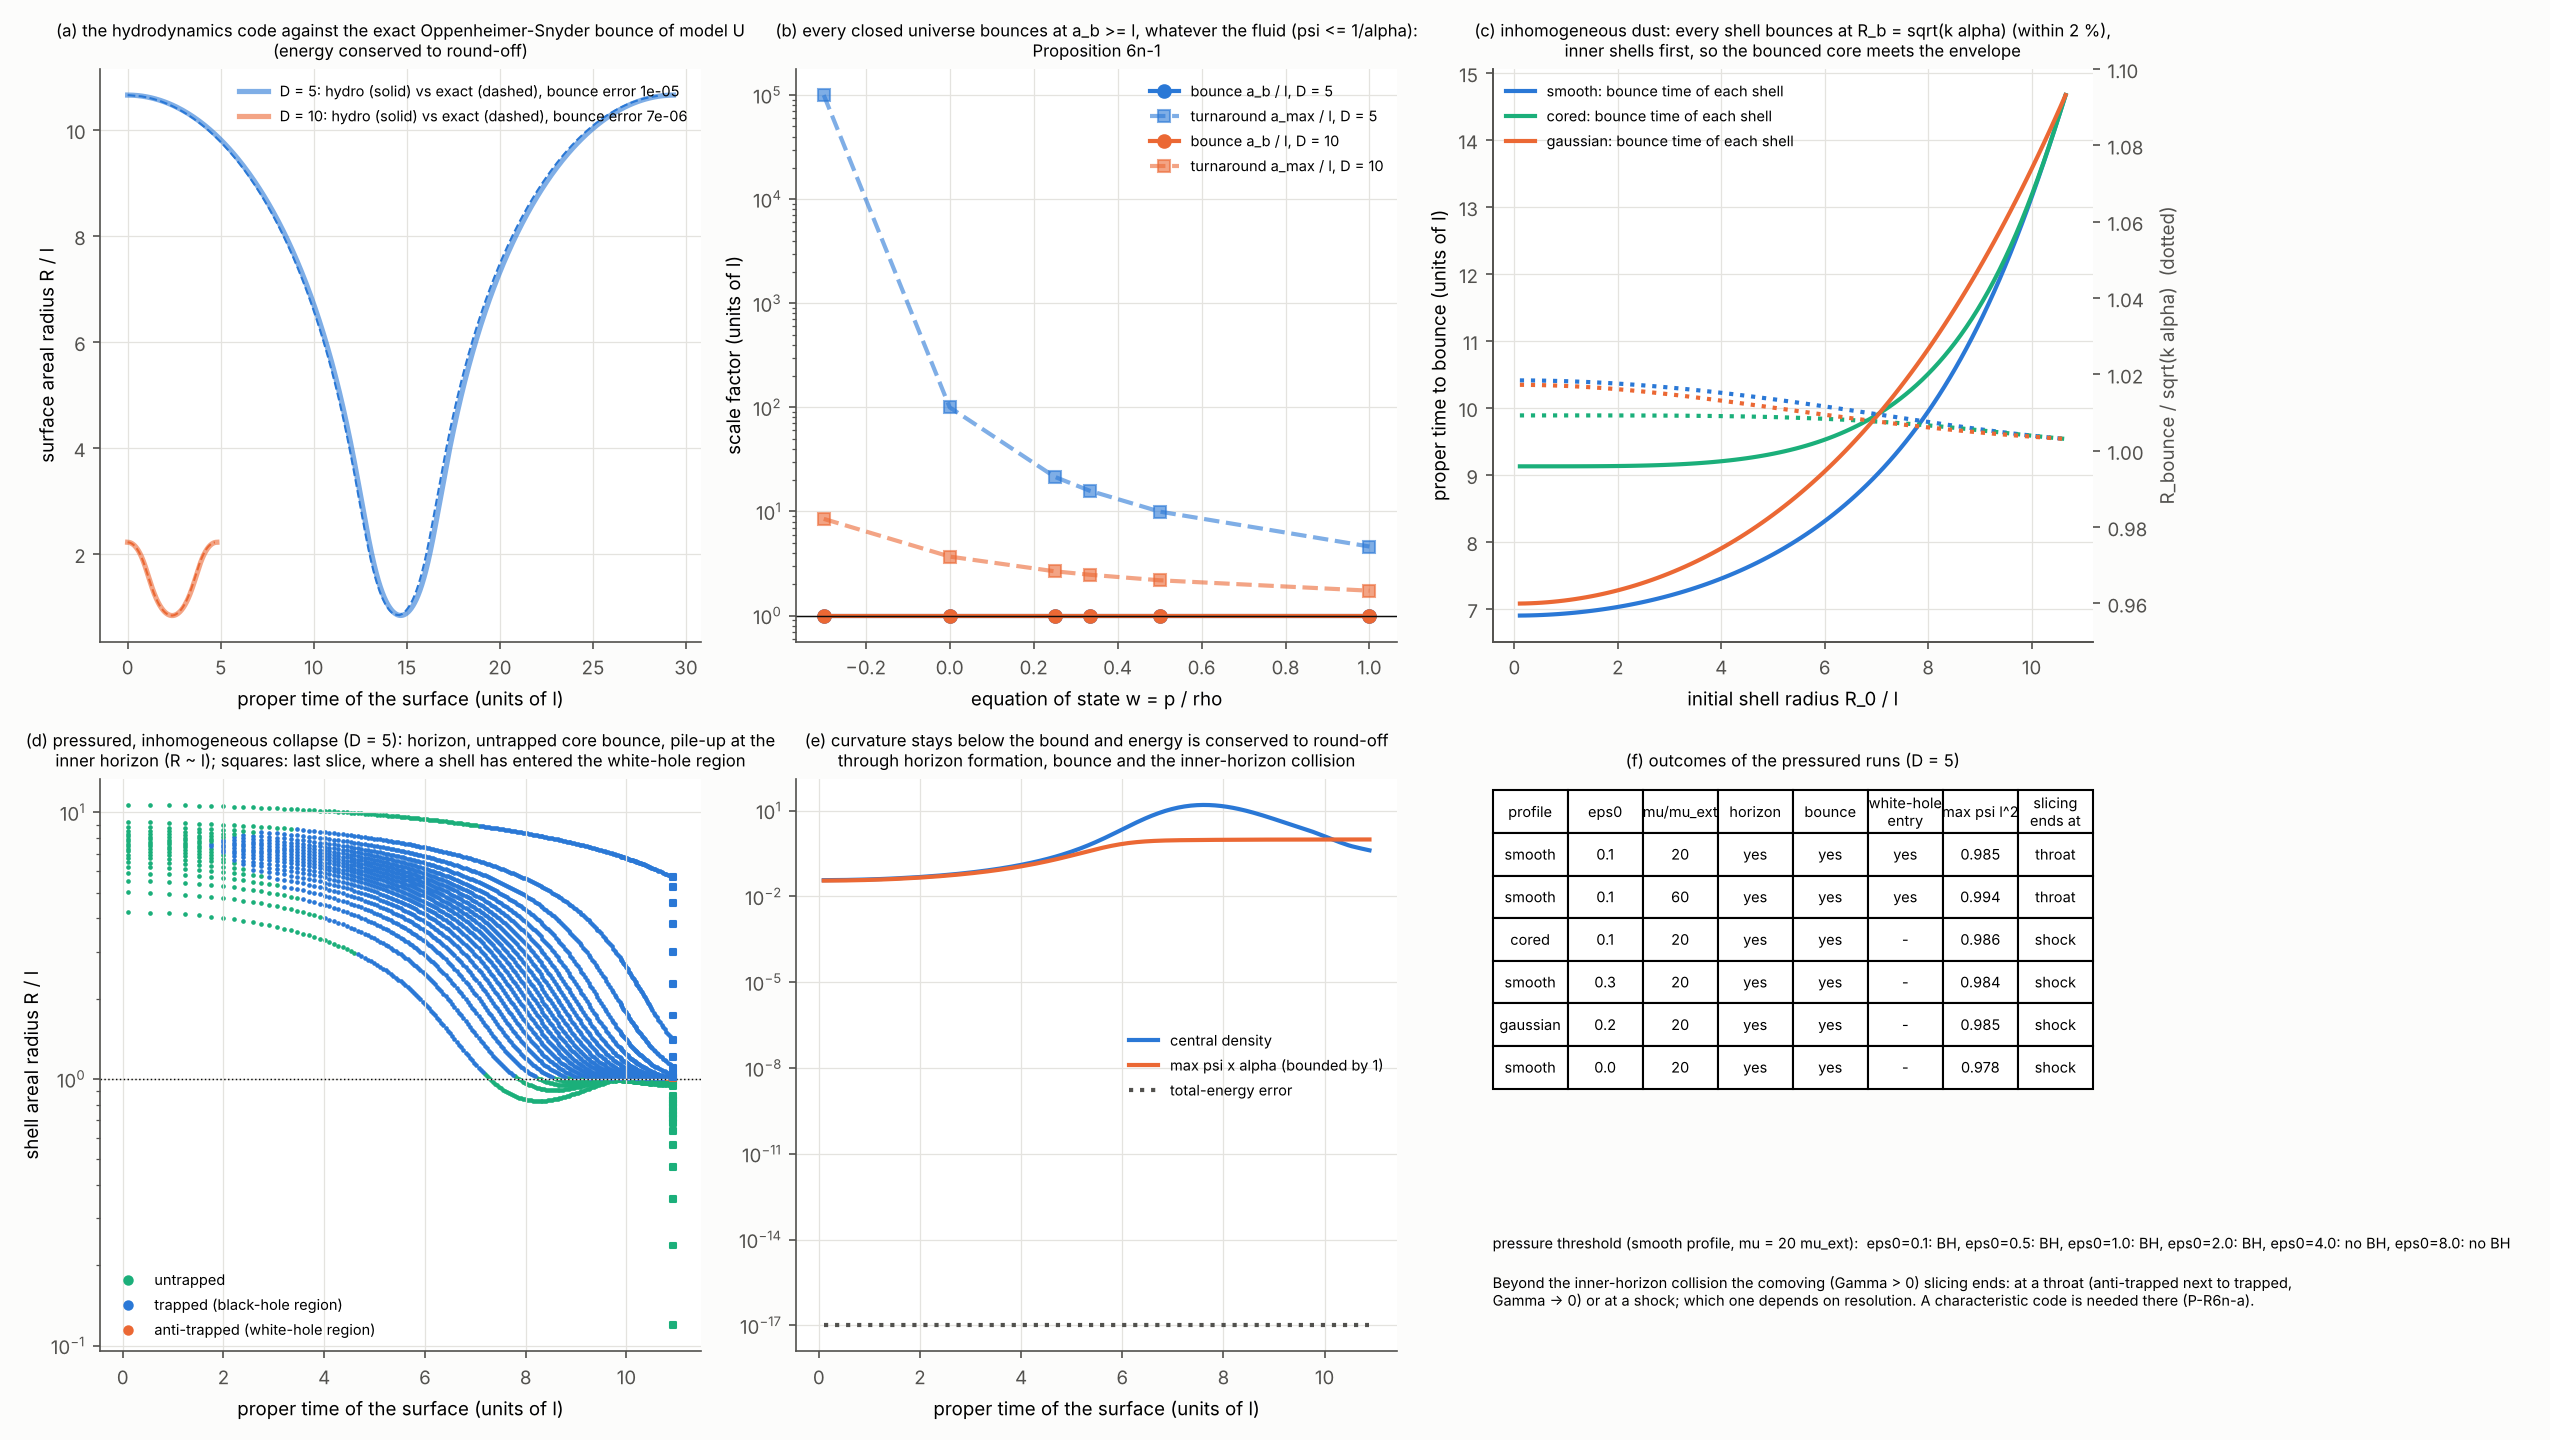
\includegraphics[width=\textwidth]{round6n.png}
\caption{Beyond idealised collapse (Round 6n): (a) hydro vs exact bounce; (b) universal bounce; (c) inhomogeneous dust; (d) pressured
collapse in a spacetime diagram; (e) bounded curvature and exact energy conservation; (f) outcomes.}\label{fig:hydro}\end{figure}

\section{Collider formation, evaporation and the daughter}
Cross-sections use NNPDF2.3 LO \cite{NNPDF23} (momentum sum $0.998$), $\hat\sigma=F_n\pi R_S^2$ with the Yoshino--Nambu factors \cite{YN03},
and the head-on trapped mass $y_n\sqrt{\hat s}$ ($y_0=1/\sqrt2$). Holes above $M_{\rm ext}$ are produced at $100$\,TeV with $30$\,ab$^{-1}$
(at least 10 events) iff $M_{\rm ext}\lesssim46$--$51$\,TeV, and are compatible with the LHC iff $M_{\rm ext}\gtrsim9$\,TeV: a window in
$c_l$ of width $\sim0.15$--$0.25$. In the evaporating model-U Vaidya geometry $f(v,r)=1-r^2\psi(\mu(v)/r^{D-1})$ with brane Stefan--Boltzmann
emission \cite{EHM00}, $\mu-\mu_{\rm ext}\propto v^{-1}$ and $r_+-r_-\propto v^{-1/2}$: the trapped region never closes, and the bounced partons
reach the boundary of the parent's chart at finite affine parameter ($\simeq2\,l$). Formation takes $\sim10^{-28}$\,s and evaporation
$10^{-26}$--$10^{-25}$\,s. An event generator built on this physics (Fig.~\ref{fig:collider}) shows that near threshold the holes are nearly
extremal and emit almost nothing (no Hawking quantum in $76$--$85\%$ of events), the remnant carrying $\simeq95\%$ of the mass.

\begin{figure}[t]\centering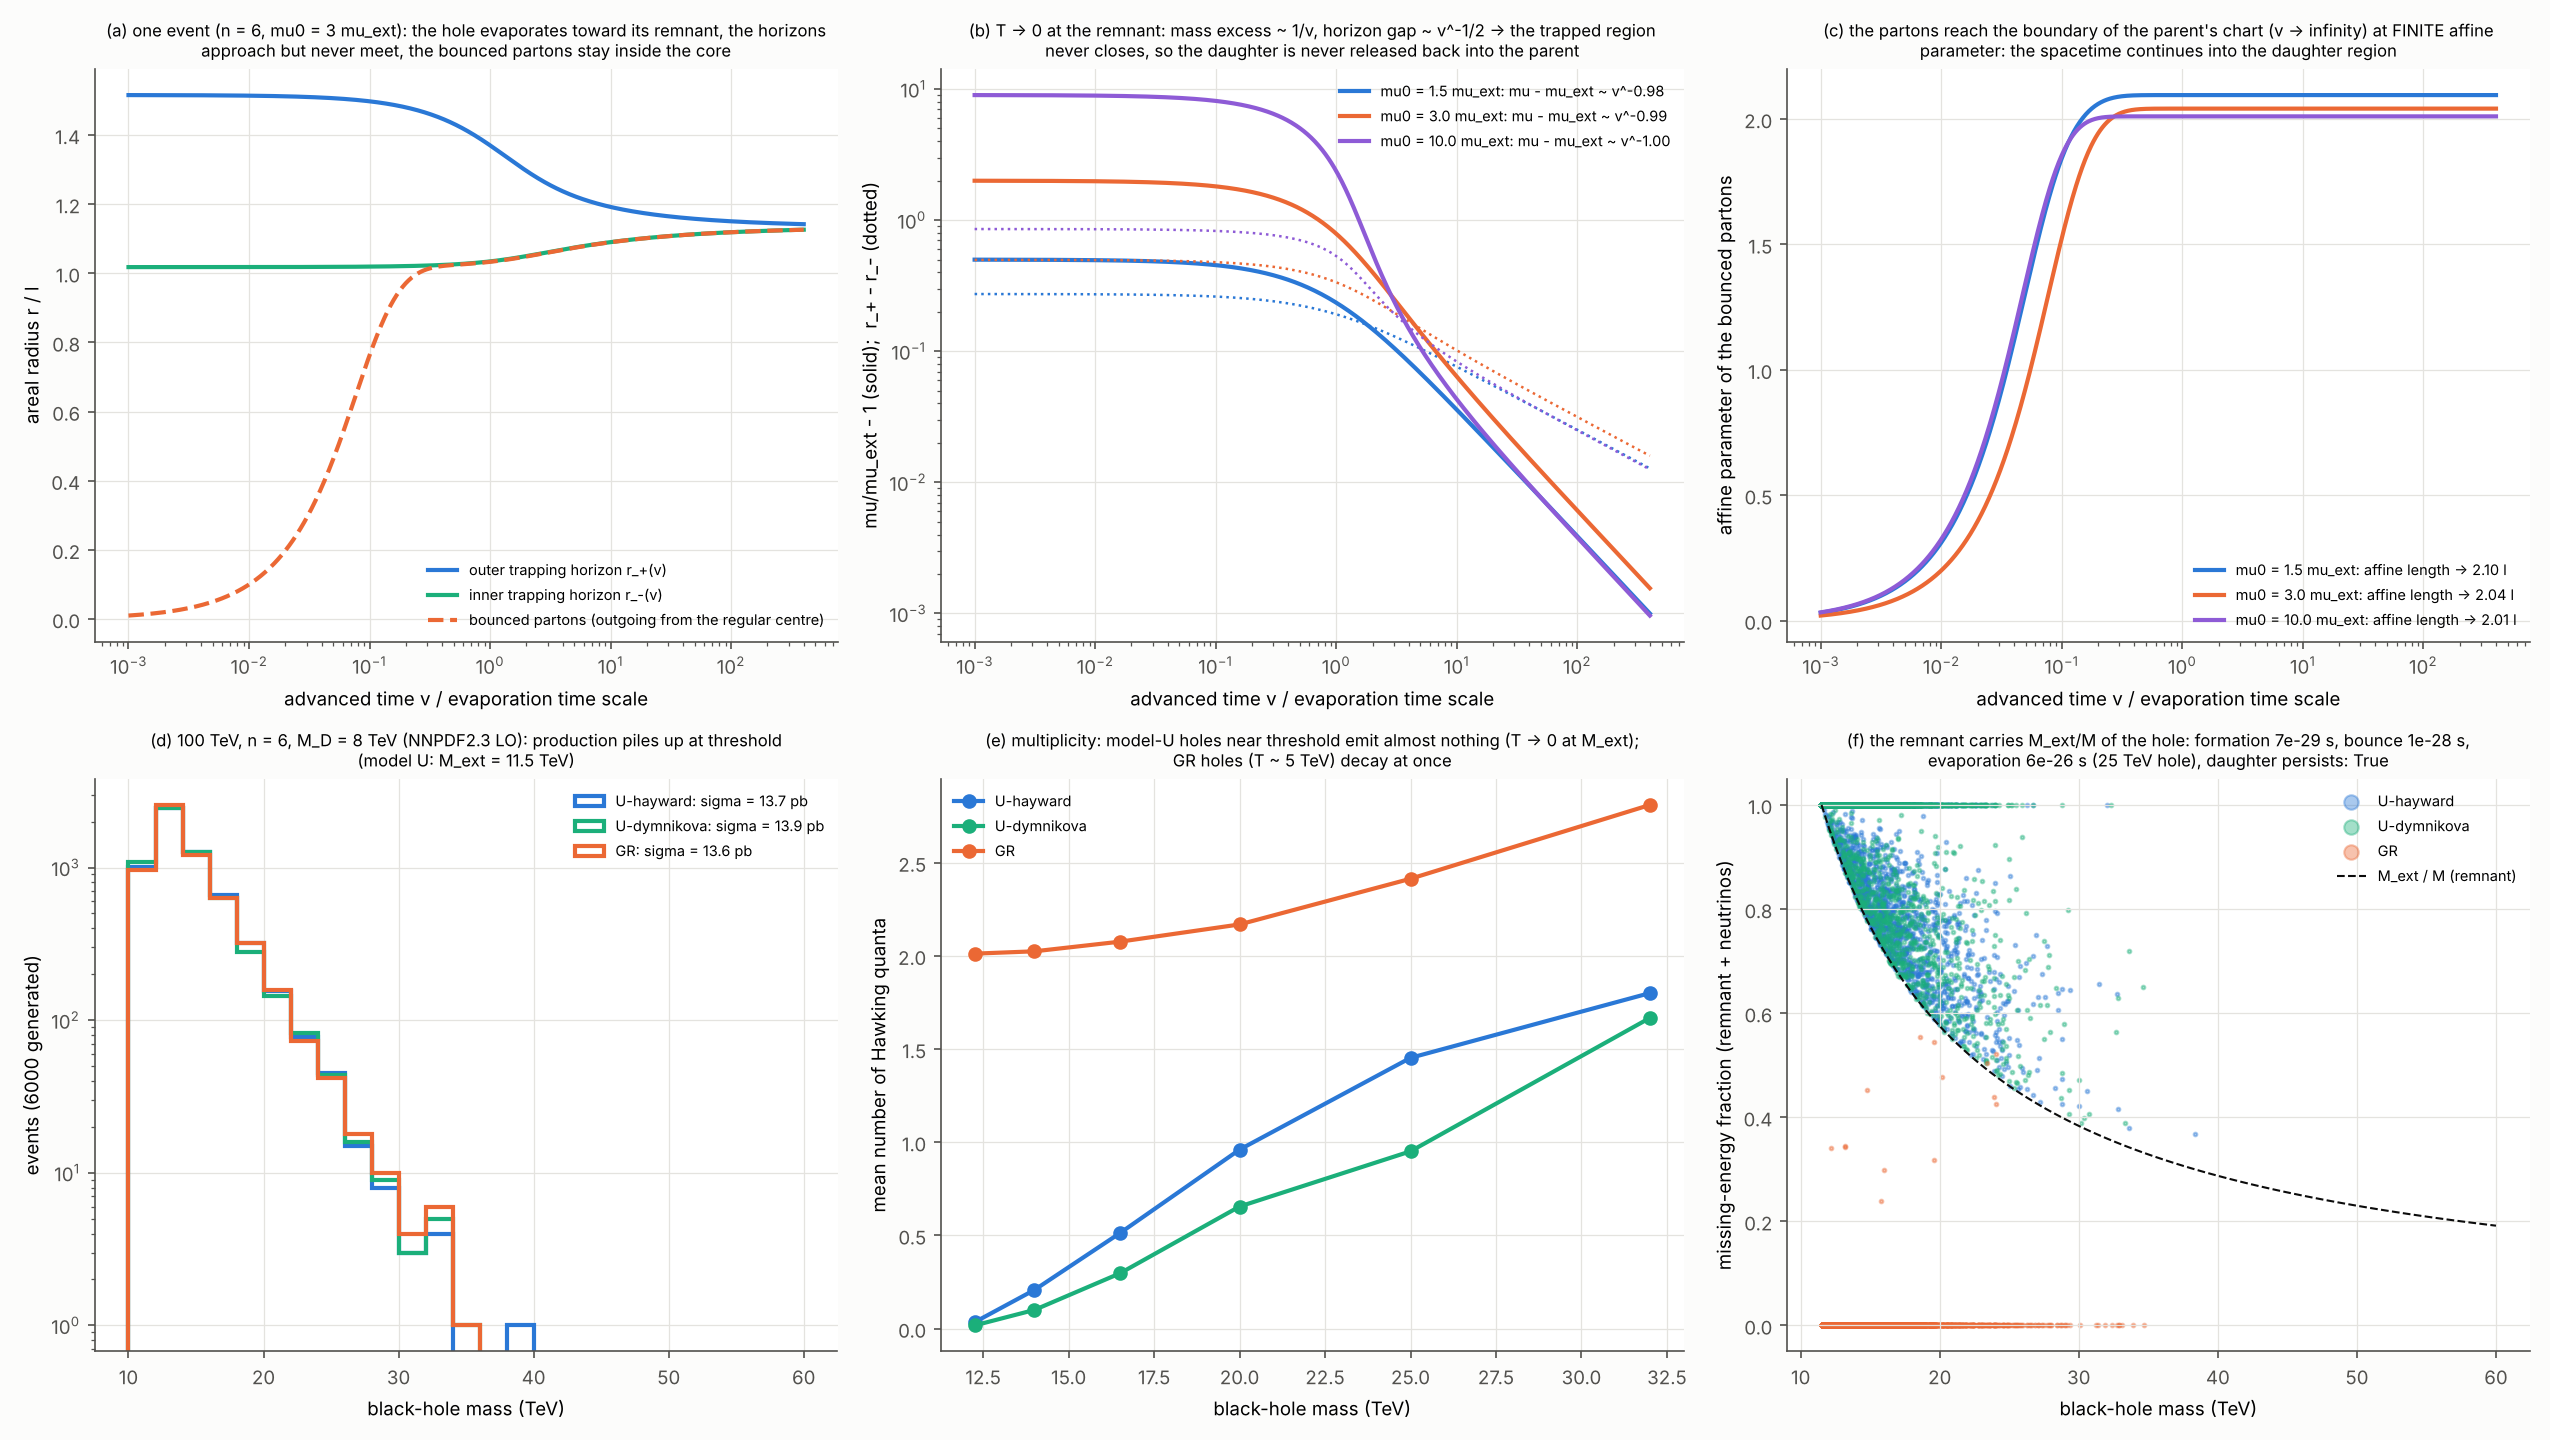
\includegraphics[width=\textwidth]{round6o.png}
\caption{One event and its observables (Round 6o): (a)--(c) evaporation toward the remnant, the horizons and the bounced partons; (d)--(f)
generator output at $100$\,TeV.}\label{fig:collider}\end{figure}

\section{Summary of results}
\begin{table}[h]\centering\small
\begin{tabular}{@{}lll@{}}\toprule
Quantity & Value & Status\\\midrule
Horizon threshold & $M_{\rm ext}=\kappa_nc_l^{\,n+1}M_D$, $\kappa_n=13$--$56$ & exact (audited)\\
Curvature bound ($D=10$) & $\max K\,l^4=188$ (Hayward), $919$ (Dymnikova), all masses & numerical (audited)\\
Closed-universe bounce & $a_b\geq l$ for every perfect fluid & proposition\\
Transient acceleration & $N\simeq\frac{D-3}{D-1}\ln(a_{\max}/l)$; $29.6$ for a stellar hole & exact (audited)\\
Lasting inflation & needs $\Lambda>\Lambda_c(C)$ (hole-density vacuum) & exact (audited)\\
Finite daughter & volume growth $(a_{\max}/l)^{D-1}$, up to $8\times10^{114}$ & exact\\
Hydrodynamic bounce & every run; $\psi\le0.994/\alpha$; energy exact; throat in 2/6 & numerical\\
Collider window & $9\lesssim M_{\rm ext}\lesssim50$\,TeV at 100\,TeV & numerical (audited)\\
Evaporation & $\mu-\mu_{\rm ext}\propto v^{-1}$, gap $\propto v^{-1/2}$, never closes & numerical (audited)\\
Near-threshold events & 0.2--0.3 quanta; remnant carries $\simeq95\%$ & Monte Carlo\\\bottomrule
\end{tabular}\caption{Main results. ``Audited'' means re-derived independently (Appendix~\ref{app:audit}).}\end{table}

\section{Limitations}
Rotation is not included (collider holes have large spin; no rotating model-U solutions are known); greybody factors are omitted; the
throat stage of inhomogeneous collapse needs a characteristic code; the threshold window depends on the unknown coefficient $c_l$; and
the daughter itself is outside $J^-(\mathcal I^+)$, so experiments can test the interior class (onset, $T(M)$, remnants) but not the daughter
directly.

\appendix
\section{Independent audit}\label{app:audit}
Each key result was re-derived by a different route (\texttt{audit6p.py}): symbolic derivations of $\mu_{\rm ext}$ and $T$ ($D=4,5,6,10$),
of $a_{\rm infl}$, of $\Lambda_c$ and of the hydrodynamic acceleration equation with its GR limit; direct Riemann-tensor computations of the
static and FRW Kretschmann formulas ($D=4,5$); the Dimopoulos--Landsberg radius from the Tangherlini mass; time integration of the interior
against quadrature; closed-form curvature against finite differences; Monte Carlo cross-sections over the raw parton grid against the
luminosity table; and an independent ODE integrator for the evaporation. The ledger is in \texttt{AUDIT\_ROUND6P.md}.

\begin{thebibliography}{99}
\bibitem{FG87} E.~Farhi, A.~H.~Guth, Phys.\ Lett.\ B \textbf{183}, 149 (1987).
\bibitem{BCH24} P.~Bueno, P.~A.~Cano, R.~A.~Hennigar, Phys.\ Lett.\ B \textbf{861} (2025), arXiv:2403.04827.
\bibitem{BCHM25a} P.~Bueno, P.~A.~Cano, R.~A.~Hennigar, \'A.~J.~Murcia, Phys.\ Rev.\ D \textbf{111}, 104009 (2025), arXiv:2412.02740.
\bibitem{BCHM25b} P.~Bueno, P.~A.~Cano, R.~A.~Hennigar, \'A.~J.~Murcia, Phys.\ Rev.\ Lett.\ \textbf{134}, 181401 (2025), arXiv:2412.02742.
\bibitem{BCHMV25} P.~Bueno, P.~A.~Cano, R.~A.~Hennigar, \'A.~J.~Murcia, A.~Vicente-Cano, arXiv:2505.09680.
\bibitem{DL01} S.~Dimopoulos, G.~Landsberg, Phys.\ Rev.\ Lett.\ \textbf{87}, 161602 (2001).
\bibitem{DKS26} F.~Di Filippo, D.~Kubiz\v{n}\'ak, A.~Srinivasan, Phys.\ Rev.\ D \textbf{114}, 044061 (2026), arXiv:2604.27980.
\bibitem{BKS21} A.~Bonanno, A.-P.~Khosravi, F.~Saueressig, arXiv:2010.04226.
\bibitem{BPS25} A.~Bonanno, D.~Panassiti, F.~Saueressig, arXiv:2507.03581.
\bibitem{NNPDF23} NNPDF Collaboration, Nucl.\ Phys.\ B \textbf{867}, 244 (2013).
\bibitem{YN03} H.~Yoshino, Y.~Nambu, Phys.\ Rev.\ D \textbf{67}, 024009 (2003).
\bibitem{EHM00} R.~Emparan, G.~T.~Horowitz, R.~C.~Myers, Phys.\ Rev.\ Lett.\ \textbf{85}, 499 (2000).
\end{thebibliography}
\end{document}
